%%%%%%%%%%%%%%%%%%%%%%%%%%%%%%%%%%%%%%%%%%%%%%%%%%%%%%%%%%%%%%%%%%%%%%%%%%%%
%  第16回 練習問題［17］〜［23］（旧 prob_p40.png / prob_p41.png / prob_p42.png）
%  ※ このファイルは記録用。実体は physics_ch16.tex に流し込み済み。
%%%%%%%%%%%%%%%%%%%%%%%%%%%%%%%%%%%%%%%%%%%%%%%%%%%%%%%%%%%%%%%%%%%%%%%%%%%%

% 第15回の［16］に続く．章単体で組んだときも番号が本体と一致するように明示しておく
\setcounter{qno}{16}

\filbreak
\Rank{A問題}

\Mon{基本事項の確認}

\hspace{1zw}以下の設問に答えよ．
\begin{komon}
\ko{1} 容器内の気体の圧力を$1.0\times 10^5\U{Pa}$に保ちながら，体積を$2.0\times 10^{-4}\U{m^3}$だけ増加させた．このとき気体が外界に対してした仕事は何$\U{J}$か．
\ko{2} 気体に$4.2\times 10^3\U{J}$の熱を加えたところ，気体は膨張し，ピストンに対して$2.4\times 10^3\U{J}$だけ仕事をした．このとき気体の内部エネルギーの増加は何$\U{J}$か．
\end{komon}

\filbreak
\Rank{B問題}

\Mon[\Sitei]{気体がする仕事}

\hspace{1zw}一定量の理想気体の状態を以下の$p-V$図の矢印の向きに静かに変化させた．このとき気体が外界にした仕事$w\U{J}$をそれぞれ求め，$p_0\U{Pa}$, $p_1\U{Pa}$, $V_0\U{m^3}$, $V_1\U{m^3}$を用いて表せ．必要があれば積分公式$\displaystyle\int\frac{1}{x}dx=\log_e|x|+C$を用いよ．

\begin{center}
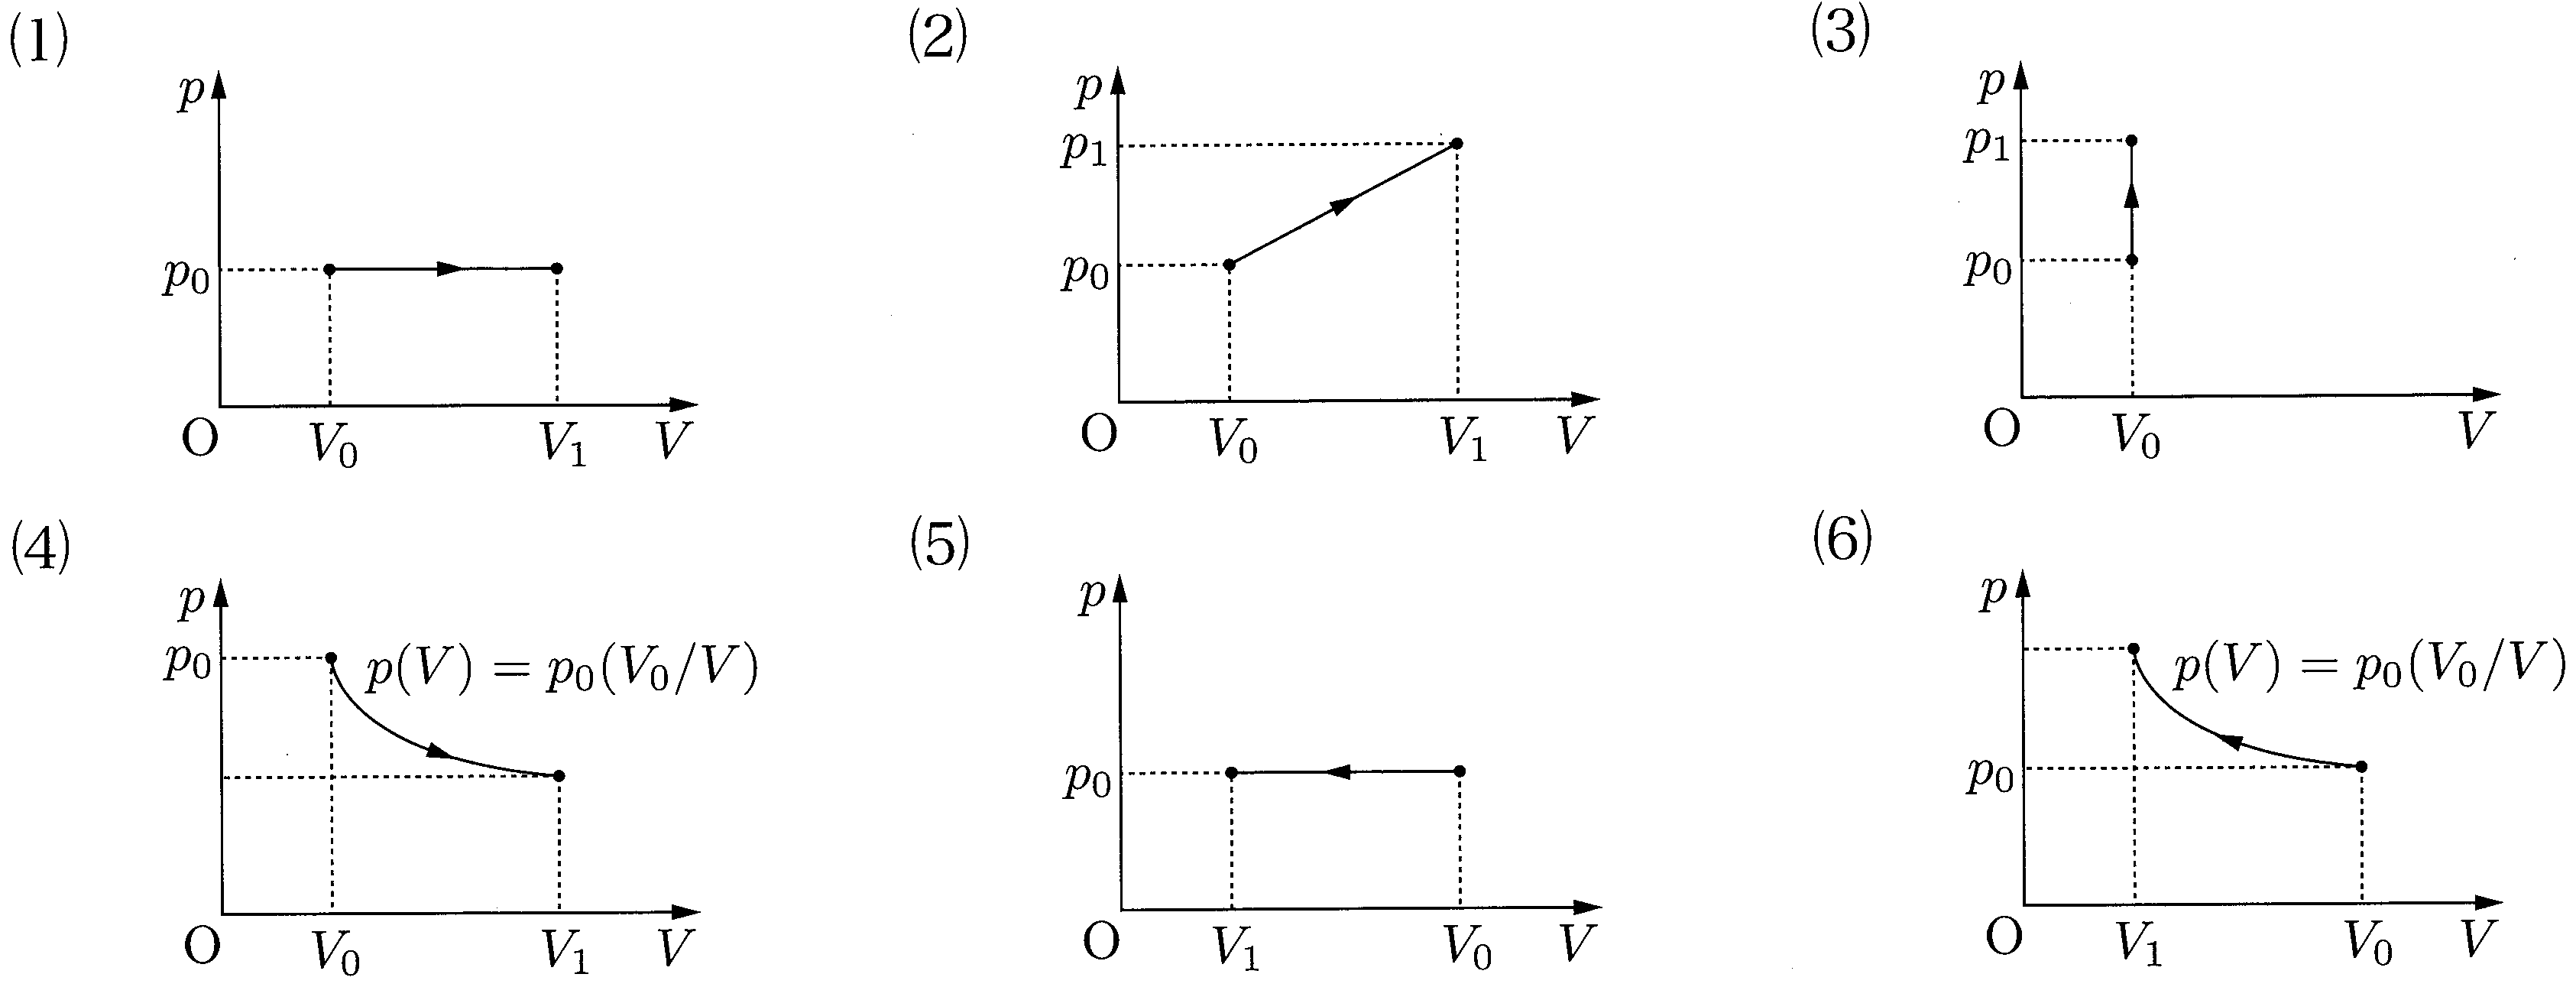
\includegraphics[keepaspectratio,width=148mm]{fig/ch16_p40_pv6.png}
\end{center}

\Mon{定圧変化}

\begin{zuright}{58mm}
\hspace{1zw}右図のように断面積$S\U{m^2}$のシリンダーの中に，なめらかに動くことのできるピストンを用いて定積モル比熱が$C_V\U{J/mol\cdot K}$の理想気体を$n\U{mol}$だけ封入した．ピストンは軽くて自由に動くことができ，ピストンの右側は大気に通じている．初め，シリンダーの底からピストンまでの距離は$l_0\U{m}$であり，また気体の温度は$T_0\U{K}$であった．
\zusep
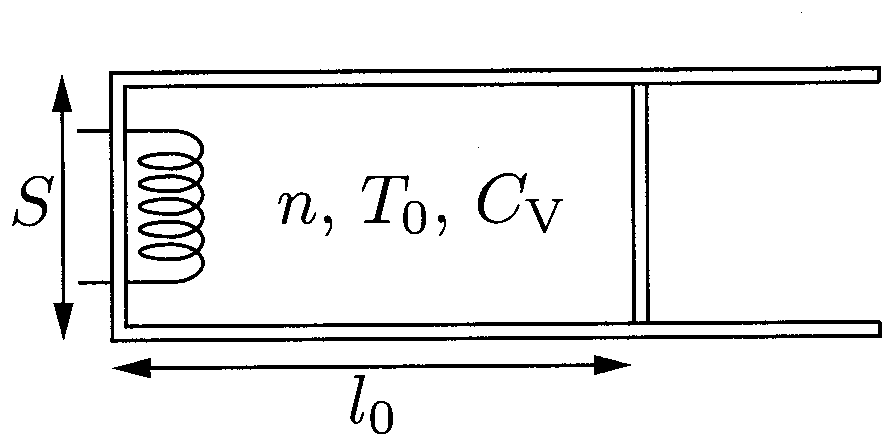
\includegraphics[keepaspectratio,width=58mm]{fig/ch16_p40_cyl.png}
\end{zuright}
\hspace{1zw}シリンダー内にはヒーターが取り付けられており，気体に対して熱を与えることができる．シリンダーおよびピストンは断熱材でできており，ヒーターによって与えた熱が大気に拡散することはないものとする．気体定数を$R\U{J/mol\cdot K}$として以下の設問に答えよ．
\begin{komon}
\ko{1} 大気圧$p_0\U{Pa}$を求めよ．
\end{komon}
\hspace{1zw}この状態から内部の気体をヒーターで少しずつ熱したところ，ピストンはゆっくりと移動し，シリンダーの底からピストンまでの距離は$l_1\U{m}$となった．
\begin{komon}
\ko{2} 終状態における気体の温度$T_1\U{K}$を求めよ．
\ko{3} この状態変化を$p-V$図で表せ．
\ko{4} この変化において，気体が外界にした仕事$w\U{J}$を求めよ．
\ko{5} ヒーターによって加えた熱量$Q\U{J}$を求めよ．
\end{komon}

\Mon{定積変化}

\begin{zuright}{58mm}
\hspace{1zw}右図のように断面積$S\U{m^2}$のシリンダーの中に定積モル比熱が$C_V\U{J/mol\cdot K}$の理想気体を$n\U{mol}$だけ封入し，ピストンの位置を固定して動かないようにした．このときのシリンダーの底からピストンまでの距離は$l_0\U{m}$であり，また気体の温度は$T_0\U{K}$であった．
\zusep
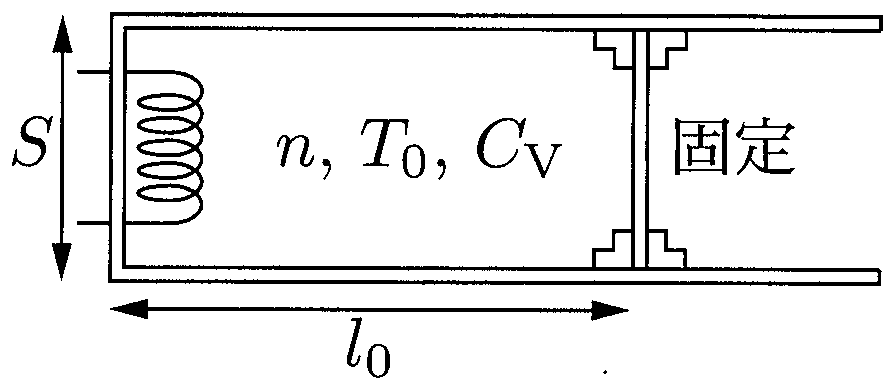
\includegraphics[keepaspectratio,width=58mm]{fig/ch16_p41_cyl.png}
\end{zuright}
\hspace{1zw}シリンダー内にはヒーターが取り付けられており，気体に対して熱を与えることができる．シリンダーおよびピストンは断熱材でできており，ヒーターによって与えた熱が大気に拡散することはないものとする．この状態からゆっくり熱し，内部の気体の温度が$T_1\U{K}$になったところで加熱を止めた．気体定数を$R\U{J/mol\cdot K}$として以下の設問に答えよ．
\begin{komon}
\ko{1} 初状態および終状態における気体の圧力$p_0\U{Pa}$, $p_1\U{Pa}$を求めよ．
\ko{2} この状態変化を$p-V$図で表せ．
\ko{3} この変化において，気体が外界にした仕事$w\U{J}$を求めよ．
\ko{4} ヒーターによって加えた熱量$Q\U{J}$を求めよ．
\end{komon}

\Mon{気体のした仕事}

\hspace{1zw}温度が$T_0\U{K}$の理想気体が$n\U{mol}$ある．この気体の温度を$T_0\U{K}$のまま一定に保ちつつ，体積を$V_1\U{m^3}$の状態$\mathrm{A}$から体積$V_2\U{m^3}$の状態$\mathrm{B}$へと膨張させる．気体定数を$R\U{J/mol\cdot K}$として以下の設問に答えよ．
\begin{komon}
\ko{1} この状態変化を$p-V$図で表せ．
\ko{2} この変化で気体が外界に対してした仕事$w$を求めよ．ただし，必要であれば積分公式$\displaystyle\int\frac{1}{x}dx=\log_e|x|+C$を用いよ．
\end{komon}

\Mon[\Sitei]{鉛直シリンダー}

\begin{zuright}{28mm}
\hspace{1zw}右図のように鉛直に立ててある断面積$S\U{m^2}$のシリンダーの中に，質量$M\U{kg}$のなめらかに動くことのできるピストンで，定積モル比熱が$C_V\U{J/mol\cdot K}$の理想気体を$n\U{mol}$だけ封入した．初め，シリンダーの底からピストンまでの高さは$l_0\U{m}$であり，大気の圧力は$p_0\U{Pa}$であった．シリンダー内にはヒーターが取り付けられており，気体に対して熱を与えることができる．シリンダーおよびピストンは断熱材でできており，ヒーターによって与えた熱が外界に拡散することはないものとする．気体定数を$R\U{J/mol\cdot K}$，重力加速度の大きさを$g\U{m/s^2}$として以下の設問に答えよ．
\zusep
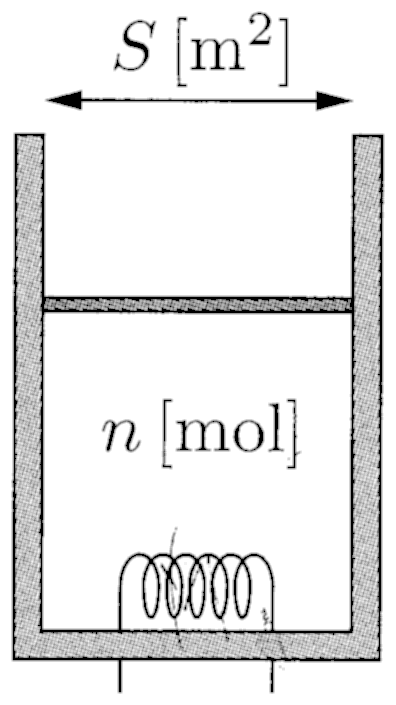
\includegraphics[keepaspectratio,width=24mm]{fig/ch16_p41_vcyl.png}
\end{zuright}
\begin{komon}
\ko{1} 初めの状態におけるシリンダー内の温度$T_0\U{K}$を求めよ．
\end{komon}
\hspace{1zw}この状態から内部の気体をヒーターで少しずつ熱したところ，ピストンはゆっくりと移動し，シリンダーの底からピストンまでの距離は$l_1\U{m}$となった．
\begin{komon}
\ko{2} 終状態における気体の温度$T_1\U{K}$を求めよ．
\ko{3} ヒーターによって気体に与えた熱量$Q\U{J}$を求めよ．
\end{komon}

\filbreak
\Rank{C問題}

\Mon{定積・定圧変化}

\begin{zuright}{34mm}
\hspace{1zw}右図のように鉛直に立ててある断面積$S\U{m^2}$のシリンダーの中に，質量$M\U{kg}$のなめらかに動くことのできるピストンで，定積モル比熱が$C_V\U{J/mol\cdot K}$の理想気体を$n\U{mol}$だけ封入した．初め，ピストンはシリンダーの底から$l_0\U{m}$の高さのところにあるストッパーにのっており，大気の圧力は$P_0\U{Pa}$，シリンダー内の気体の温度は$T_0\U{K}$であった．シリンダー内にはヒーターが取り付けられており，気体に対して熱を与えることができる．シリンダーおよびピストンは断熱材で出来ており，ヒーターによって与えた熱が大気に拡散することはないものとする．気体定数を$R\U{J/mol\cdot K}$，重力加速度の大きさを$g\U{m/s^2}$として以下の設問に答えよ．
\zusep
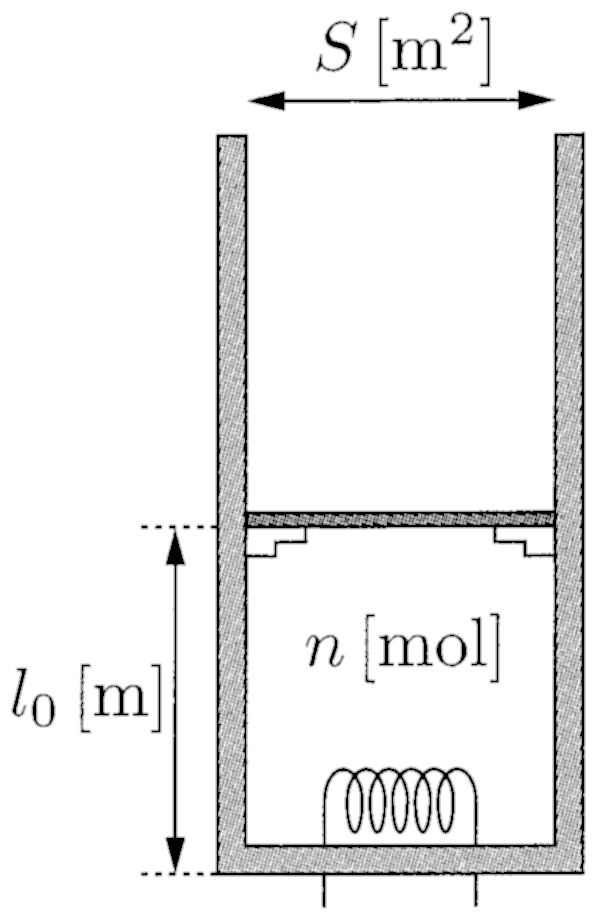
\includegraphics[keepaspectratio,width=30mm]{fig/ch16_p42_vcyl.png}
\end{zuright}
\begin{komon}
\ko{1} 初めの状態におけるシリンダー内の気体の圧力$p'\U{Pa}$を求めよ．
\end{komon}
\hspace{1zw}この状態から内部の気体をヒーターで少しずつ熱したところ，ピストンは静止したままであったが，しばらくすると動き始めた．さらに加熱を続けると，ピストンはゆっくりと上昇し，シリンダーの底からピストンまでの距離は$l_1\U{m}$となった．
\begin{komon}
\ko{2} ピストンが動き始めたときのシリンダー内の気体の温度$T_1\U{K}$を求めよ．
\ko{3} 終状態における気体の温度$T_2\U{K}$を求めよ．
\ko{4} ピストンが動き始める前と後とに分けて考えることに注意して，最初の状態からこの状態に至るまでの間にヒーターによって気体に与えられた総熱量$Q\U{J}$を求めよ．
\end{komon}
